% !TeX root = ../main.tex
\section{Zusammenhalt des Netzwerks}
\label{sec:zusammenhalt}

Nachdem Kapitel~\ref{sec:zentralitaet} gezeigt hat, wer im Netz zentral
ist, fragen wir nun, was das Netz zusammenhält. Sind es einzelne Athleten
oder die Veranstaltungen, an denen sie sich treffen? Grundlage ist wieder
das Arbeitsnetz mit 13\,156 Athleten und 357\,219 Kanten.

\subsection{Kennzahlen und Nullmodell}
Das Arbeitsnetz ist mit einer Density von 0,0041 sehr dünn, aber lokal
stark vernetzt. Das Clustering, also der mittlere Anteil verbundener
Nachbarspaare, beträgt 0,49. Zwischen zwei Athleten der Giant Component
liegen höchstens elf Schritte (Diameter). Die Degree-Zentralisierung von
0,037 und die Betweenness-Zentralisierung von 0,018 sind sehr tief. Kein
einzelner Athlet dominiert das Netz.

Ein Teil dieser Struktur entsteht durch die Projektion, da jeder
Veranstaltungstag seine Athleten vollständig verbindet. Das gewöhnliche
Configuration Model berücksichtigt das nicht und ist deshalb kein fairer
Vergleich. Wir verwenden deshalb das bipartite Configuration Model, das die
Projektion berücksichtigt. Dafür verteilen wir die Athleten 100-mal
zufällig auf die Teilnahmen. Jeder Veranstaltungstag behält seine Grösse,
jeder Athlet seine Zahl an Tagen. Die Zahl der Begegnungen bleibt damit
gleich, nur ihre Verteilung auf Athletenpaare ist zufällig. Danach
projizieren und filtern wir wie im Original. Die Nullhypothese
lautet, dass die Struktur allein aus diesen Grössen entsteht.

\begin{table}[H]
  \centering
  \caption{Arbeitsnetz und Nullmodell mit zufällig verteilten Teilnahmen
  (100 Referenz-Netzwerke). Eigene Auswertung.}
  \label{tab:nullmodell}
  \begin{tabular}{@{}lrrr@{}}
    \toprule
    & Arbeitsnetz & Nullmodell Mittel & Nullmodell Maximum \\
    \midrule
    Kanten & 357\,219 & 35\,930 & 36\,692 \\
    Clustering & 0,49 & 0,04 & 0,04 \\
    Anteil Giant Component & 96,6\,\% & 65,7\,\% & 66,6\,\% \\
    \bottomrule
  \end{tabular}
\end{table}

Tabelle~\ref{tab:nullmodell} zeigt einen deutlichen Unterschied. Das
Arbeitsnetz hat rund zehnmal so viele Kanten wie die Referenz-Netzwerke,
und keines erreicht einen der beobachteten Werte ($p < 0{,}01$,
$\alpha = 0{,}05$). Wiederholte Begegnungen sind also kein Zufall.
Dieselben Athleten treffen sich immer wieder, etwa an nationalen
Meisterschaften und regelmässigen internationalen Wettkämpfen. Das passt zu
den nationalen Communities aus Kapitel~\ref{sec:communities}.

\subsection{Robustheit}
Abbildung~\ref{fig:robustheit} zeigt, wie sich die Giant Component
verändert, wenn wir schrittweise Athleten oder Veranstaltungstage
entfernen. Athleten entfernen wir nach absteigender Betweenness aus
Kapitel~\ref{sec:zentralitaet}, nach Degree oder zufällig. Bei den
Veranstaltungstagen beginnen wir mit den internationalsten, gemessen an der
Zahl der Nationen am Tag, mit den grössten oder mit zufälligen Tagen. Nach
jedem Schritt wird neu projiziert.

\begin{figure}[H]
  \centering
  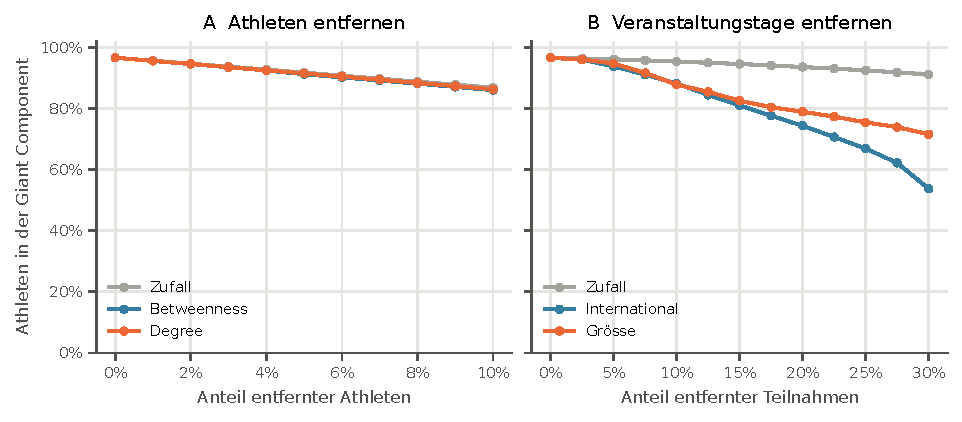
\includegraphics[width=\textwidth]{07_robustheit.pdf}
  \caption{Anteil aller Athleten in der Giant Component beim Entfernen von
  Athleten (A) und Veranstaltungstagen (B). In B zeigt die x-Achse den
  Anteil entfernter Teilnahmen. Grau: Mittel von zehn zufälligen Reihenfolgen, die sich um höchstens
  1,4 Prozentpunkte unterscheiden. Eigene Auswertung.}
  \label{fig:robustheit}
\end{figure}

Das Entfernen einzelner Athleten schadet dem Netz kaum. Auch ohne die 10\,\%
mit der höchsten Betweenness bleiben 86,0\,\% aller Athleten in der Giant
Component, bei zufällig entfernten Athleten 86,8\,\%. Verloren gehen fast
nur die entfernten Athleten selbst. Auch die 184 Cut-Vertices trennen
jeweils höchstens drei Athleten ab, im Median einen. Sie binden einzelne
Athleten am Rand an, ein verwundbarer Kern existiert nicht.

Ganz anders bei den Veranstaltungstagen. Fehlen die internationalsten Tage
mit zusammen 30\,\% der Teilnahmen, bleiben nur 53,7\,\% der Athleten in
der Giant Component, bei zufälligen Tagen 91,1\,\%. Die grössten Tage
tragen zwar mehr Kanten, ihr Entfernen zerlegt das Netz aber weniger
(71,5\,\%). Entscheidend ist also nicht die Grösse eines Tages, sondern
dass er Athleten vieler Nationen zusammenbringt. Internationale
Meisterschaften wie die Weltmeisterschaft 2009 in Rom mit 105 Nationen an
einem Tag halten das Netz zusammen. Das erklärt auch, warum ihr Kern in
Kapitel~\ref{sec:communities} und die Eigenvector-Spitze in
Kapitel~\ref{sec:zentralitaet} so hervortreten.

\subsection{Generationen im Vergleich}
Tabelle~\ref{tab:generationen_kennzahlen} vergleicht die Teilnetze der vier
Generationen aus Kapitel~\ref{sec:communities} in zeitlicher Reihenfolge.
Da die Density von der Grösse abhängt, betrachten wir vor allem den
mittleren Grad.

\begin{table}[H]
  \centering
  \caption{Teilnetze der Generationen im Arbeitsnetz, sortiert nach Jahrgang.
  Mittlerer Grad: durchschnittliche Zahl Nachbarn innerhalb der Generation.
  Zentralisierung: Degree-Zentralisierung nach Freeman. Eigene Auswertung.}
  \label{tab:generationen_kennzahlen}
  \begin{tabular}{@{}lrrrrrr@{}}
    \toprule
    & Jahrgang & Athleten & Mittlerer Grad & Clustering & Diameter & Zentralisierung \\
    \midrule
    C4 & 1978 & 1\,175 & 27,9 & 0,52 & 9 & 0,11 \\
    C2 & 1988 & 1\,881 & 67,7 & 0,53 & 7 & 0,21 \\
    C3 & 1996 & 1\,304 & 52,9 & 0,60 & 7 & 0,23 \\
    C1 & 2002 & 2\,064 & 50,1 & 0,54 & 7 & 0,18 \\
    \bottomrule
  \end{tabular}
\end{table}

Die Generation mit Jahrgang 1988 (C2) ist am dichtesten vernetzt. Ein
Drittel ihrer Teilnahmen fällt in die Jahre 2008 und 2009, in denen der
Datensatz bereits in Kapitel~\ref{sec:daten} einen Anstieg zeigt. Ihre
Bestleistungen konzentrieren sich damit auf wenige Saisons und dieselben
Meisterschaften, allen voran die Weltmeisterschaft 2009 in Rom. Die
zentralsten Athleten von C2 sind Sheng-Yo Ting, Andrejs Duda und Grant
Beahan, also dieselben wie an der Eigenvector-Spitze in
Kapitel~\ref{sec:zentralitaet}. Auch in C3 prägen Athleten kleinerer
Nationen wie Nordmazedonien, Nicaragua oder der Philippinen die Spitze.
Wenige Athleten, die an vielen grossen Meisterschaften starten, erklären so
die höhere Zentralisierung dieser beiden Generationen.

Die älteste Generation C4 ist am losesten verbunden. 77\,\% ihrer
Teilnahmen liegen vor 2005, im gesamten Datensatz sind es nur 5\,\%. Ein
Athlet von C4 hat im Median nur sieben gespeicherte Veranstaltungstage, in
C2 sind es 13. Die geringe Vernetzung von C4 spiegelt deshalb vor allem,
dass ältere Bestleistungen seltener erfasst sind. Das Clustering ist in
allen Generationen ähnlich hoch, da es vor allem aus der Projektion
entsteht.
